\documentclass[11pt,aspectratio=1610,dvipsnames]{beamer}
\graphicspath{{figs/}}
\usetheme{default}
\usepackage{DasBeamerPaket}
\usepackage{animate}
\usepackage{lastpage}
\setbeamercolor{section in toc}{fg=NavyBlue}
\setbeamercolor{frametitle}{fg=NavyBlue}
\captionsetup[figure]{labelfont=bf}
\captionsetup[table]{labelfont=bf}
\setbeamertemplate{caption}[numbered]
\begin{document}
\author{{\Large Dominic Schüchter}\\ \scriptsize \href{mail:dschuechter@uni-bonn.de}{\faEnvelope  \hspace*{0.1cm}dschuechter@uni-bonn.de} {\color{black}$|$} \href{https://github.com/dschuechter}{\faGithub  \hspace*{0.1cm}dschuechter}}
\title{Bayesian model selection}
\subtitle[Seminar physics760]{\textsc{Seminar physics760-Computational Physics}}
\logo{
\includegraphics[width=1cm]{UniBonnLogo}\vspace{235pt}\hspace{8pt}}

\date{\includegraphics[width=1.3cm]{institutelogo}\hspace{10px}
\includegraphics[width=1.3cm]{UniBonnLogo}}
\date{\includegraphics[width=8cm]{Titelbild.png}}


\setbeamertemplate{footline}[text line]{\parbox{0.3\linewidth}{\vspace*{-9pt}\textcolor{white} \insertsection  \hfill} \parbox{0.7\linewidth}{\vspace*{-8pt} \textcolor{white} {\hfill\insertshorttitle\hfill\insertshortsubtitle  \hfill \insertpagenumber/\pageref{LastPage}}}}

\addtobeamertemplate{footline}{ \makebox[0pt][l]{\hspace{-1cm}
		\raisebox{0cm}[0pt][0pt]{\colorbox{gray!15!black}{\phantom{{\large TEXTTEXTTEXTTEXTTEXTTEXTTEXTTEXTTEXTTEXTTEXTTEXTTEXTTEXTTEXTTEXTTEXTTEXTTEXTTEXTTEXTTEXTTEXTTEXTTEXTTEXTTEXTTEXTTEXTTEXTTEXTTEXTTEXTTEXTTEXTTEXTTEXTTEXTTEXTTEXT}}}}}}

\setbeamercovered{transparent}
\setbeamertemplate{navigation symbols}{}
\setbeamertemplate{frametitle}[default][left,leftskip=0.5cm]
%
\setbeamertemplate{itemize item}{\color{black}$\blacktriangleright$}
\setbeamertemplate{section in toc}[sections numbered]
\captionsetup{font=scriptsize,labelfont=scriptsize}



\begin{frame}[plain]
	\setcounter{page}{0}
	\centering
	{\Large \color{MidnightBlue}{\textsc{Bayesian} model selection}}\\
	{Seminar physics760 -- Computational Physics}
	\vfill
	
	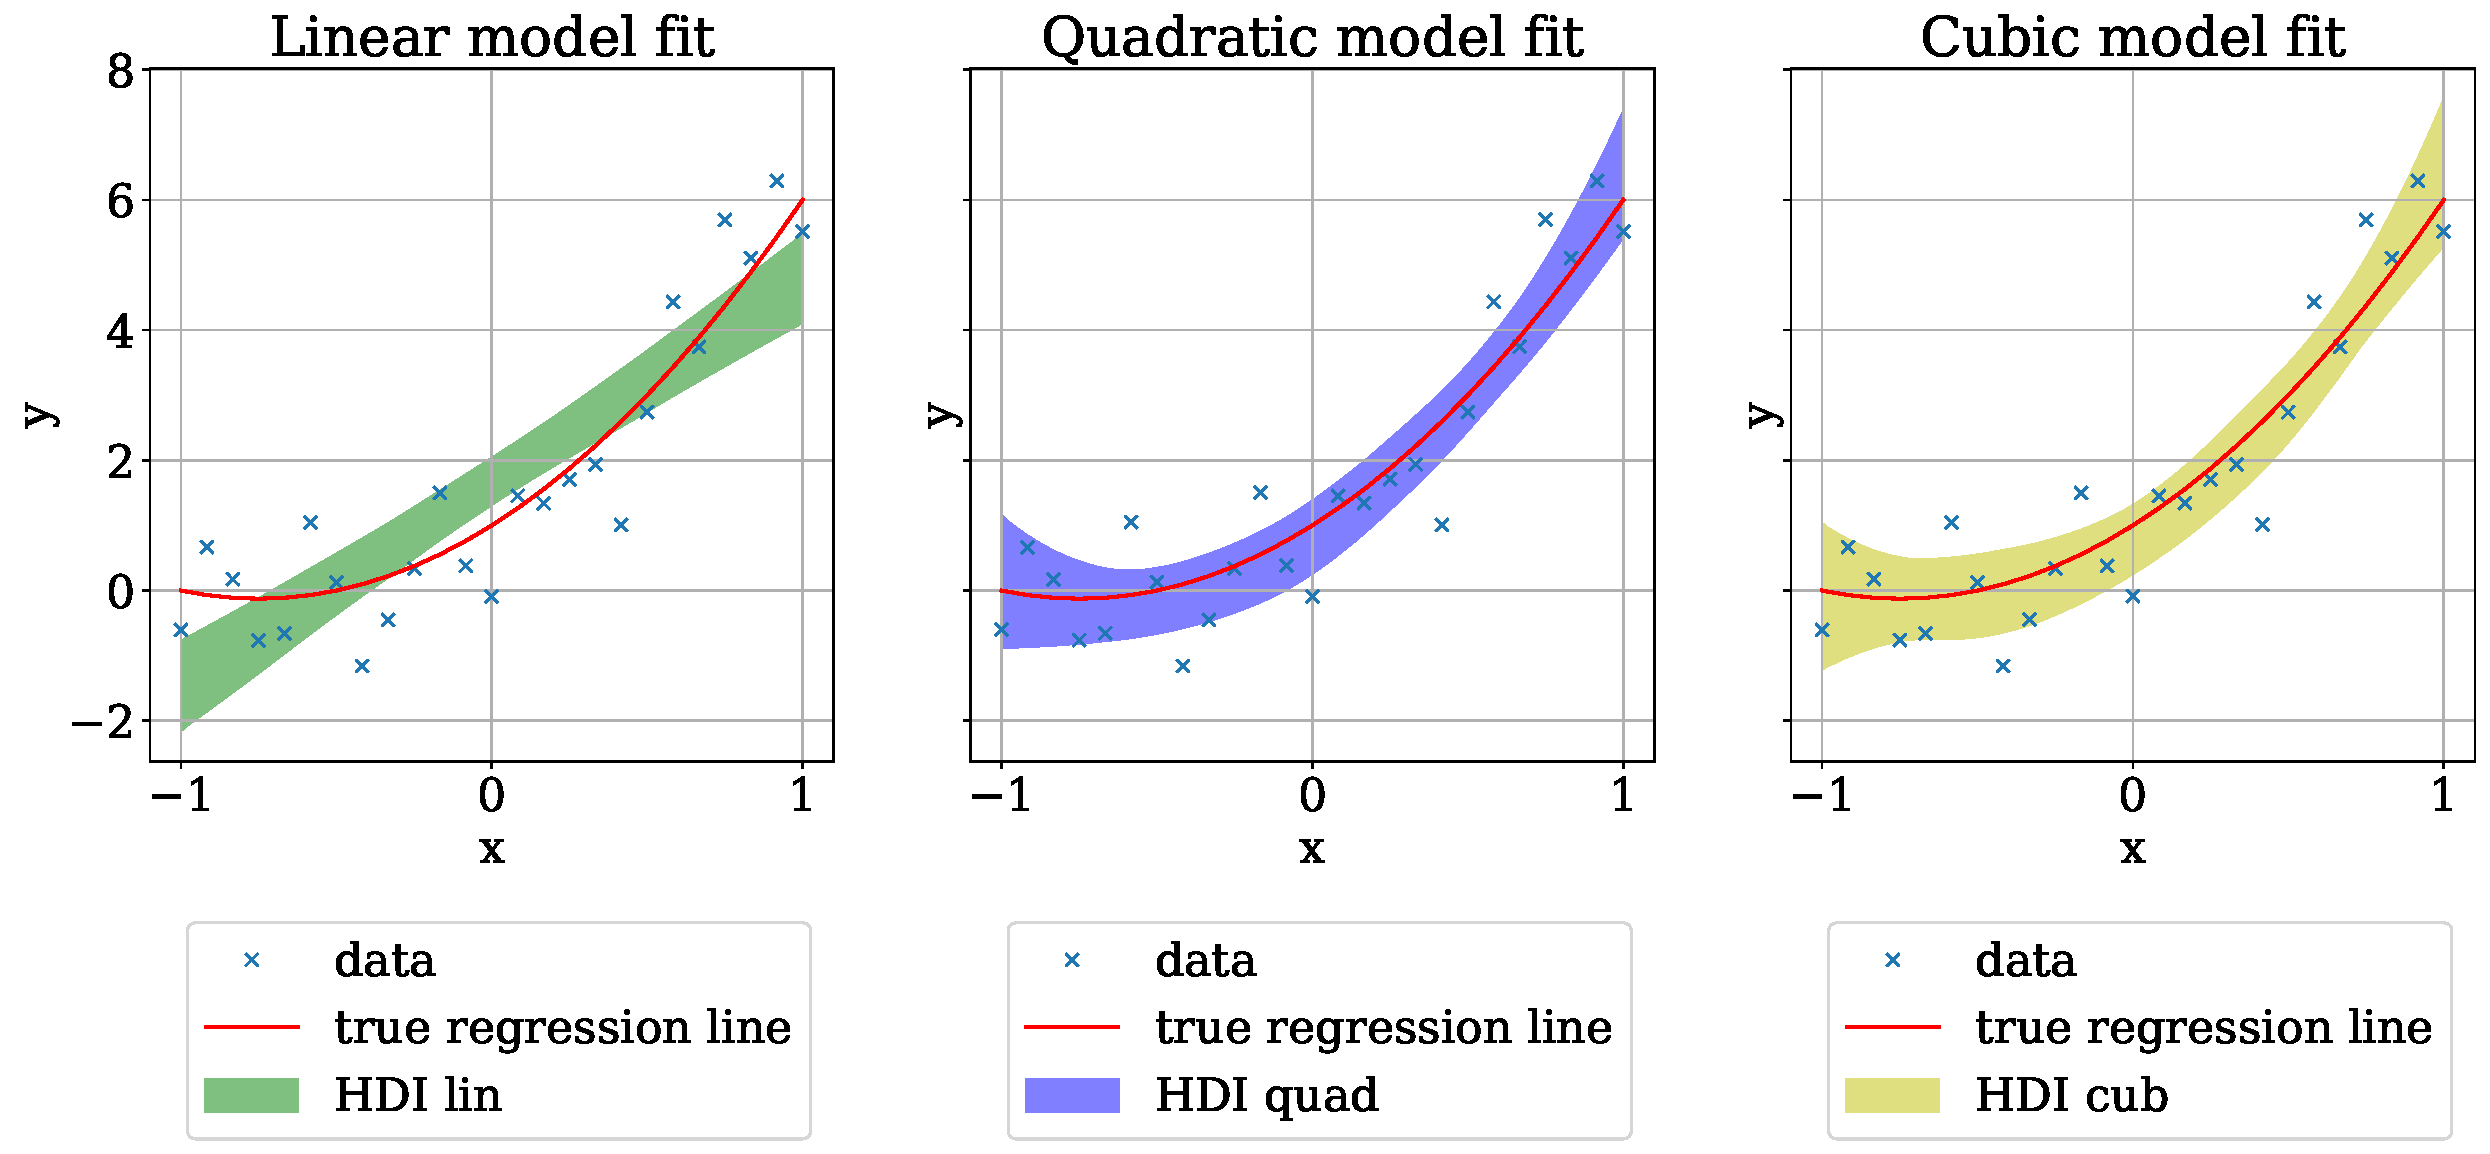
\includegraphics[width=0.5\linewidth]{HDI_sigma_07a}
	\vfill
	\begin{minipage}{\linewidth}
		\centering
		\begin{minipage}{0.45\linewidth}
			\centering
			\textsc{Dominic Schüchter}\\
			\scriptsize \href{mailto:dschuechter@uni-bonn.de}{\faEnvelope  \hspace*{0.1cm}dschuechter@uni-bonn.de} {\color{black}$|$} \href{https://github.com/dschuechter}{\faGithub  \hspace*{0.1cm}dschuechter}\\
		\end{minipage}
%		$|$
		\begin{minipage}{0.45\linewidth}
			\centering
			\textsc{Jakob Krause}\\
			\scriptsize \href{mailto:krause@hiskp.uni-bonn.de}{\faEnvelope  \hspace*{0.1cm}krause@hiskp.uni-bonn.de} {\color{black}$|$} \href{https://github.com/krausejm}{\faGithub  \hspace*{0.1cm}krausejm}\\
		\end{minipage}
	\vspace{.5cm}
	
	Tutor: \textsc{Andreas Wirzba}\\
	\scriptsize \href{mailto:a.wirzba@fz-juelich.de}{\faEnvelope  \hspace*{0.1cm}a.wirzba@fz-juelich.de}
	\end{minipage}
	\vspace{0.5cm}
	
	19.03.2021
	 
	
%	  \makebox[0pt][l]{\hspace{-7cm}
%	 	\raisebox{0.2cm}[0pt][0pt]{%
%	 		
\includegraphics[width=2.5cm]{pics/UniBonnLogoWithTextMod.png} }}
 		
\end{frame}

%\begin{frame}[plain]
%	\maketitle
%	\setcounter{page}{0}
%\end{frame}

\section*{Introduction}
\begin{frame}{Introduction}
	\begin{tcolorbox}[colback=black!5,colframe=gray!15!black,title=\textsc{Bayes'} Theorem] 
\end{tcolorbox}
\end{frame}


\section*{Table of Contents}

\begin{frame}{Table of Contents}
	\tableofcontents
\end{frame}



\section{Summary}
\begin{frame}{Summary}
	\begin{tcolorbox}[colback=black!5,colframe=gray!15!black,title=, width=\linewidth]
		\begin{itemize}
			\item 
		\end{itemize}
	\end{tcolorbox}
\end{frame}

\section*{References}
\begin{frame}[allowframebreaks]{References}
	\setbeamertemplate{bibliography item}[text]
	\bibliographystyle{plainnat}
	\bibliography{refs}
\end{frame}

\end{document}